\skriptsection{Multilayer Neural Networks / Multilayer Perceptrons}{282}
  Multilayer Neural Networks (MNN) implement linear discriminants but in space where inputs have been mapped non-linearly.
 
 \skriptsubsection{Feedforward Operation / Classification}{284}
 The feedforward operation is used to calculate  the most probable class given a test sample.\\
 
    \begin{wrapfigure}{l}{10cm}
        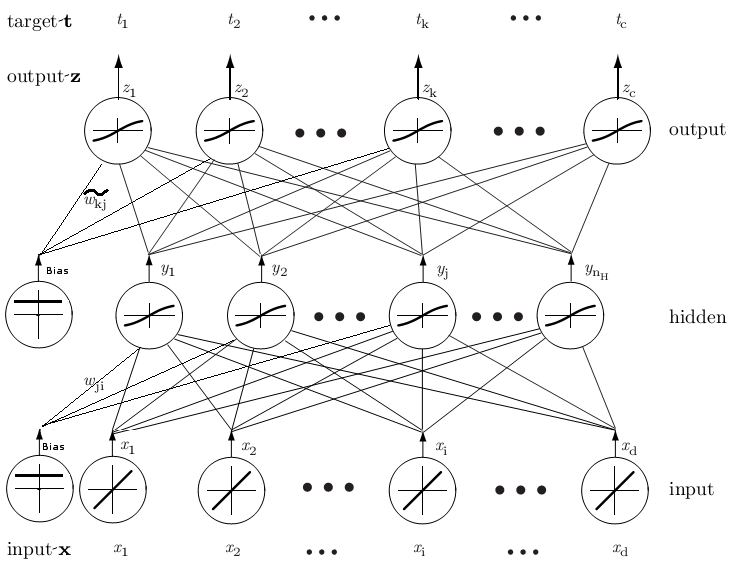
\includegraphics[width=10cm]{./images/feedforwardOperation.png}
    \end{wrapfigure}

  \textbf{Input Layer (x)}: Represent the input $\bm{ x}$ and has $d$ linear input nodes. 
  To standardize the inputs, the mean value of the training set has to be subtracted and it has to 
  be divided by its variance.\\
  
  \textbf{Output Layer (z)}: Represent the classes $\bm{ z}$ and has the dimension $c$. This nodes can have a nonlinear weight function.\\
  
  \textbf{Hidden Layer}: Between output and input. There can be more than one hidden layer. 
  Has most of the time non-linear weight function. The number of this nodes $n_H$ is a design parameter.\\
  
  \textbf{Modifiable weights/ Synapse} $\bm{ w_{ji}}$ and  $\bm{\tilde{w}_{kj}}$: 
  connect input $(i)$ with hidden $(j)$ node and hidden $(j)$ with the output $(k)$ node, respectively.  \\
  
  \textbf{Bias Unit}: Used to model a bias in each layer. One bias unit is connected to each layer except the input layer: 
  $\omega_{j0}$ input bias, $\tilde \omega_{k0}$ hidden bias.\\
  
  \textbf{Net Activation}: The sum of all weighted inputs of a node is called net activation or net. 
  \begin{align*}
      \mathrm{net}_j = \sum\limits_{i=0}^d x_i w_{ji} = \bm w_j^T\bm x \qquad\text{for hidden nodes} &&
      \tilde{\mathrm{net}}_k = \sum\limits_{j=0}^{n_H} y_j \tilde{w}_{kj} = \bm{ \tilde{w}}_k^T\bm y  \qquad\text{for output nodes}
  \end{align*}

  \textbf{Activation Function (Neuron)}: Every node has an \em activation function $f(\cdot)$\em. 
  $y_j=f_j(net_j)$ for hidden nodes, $z_k=\tilde f_k(\tilde{net}_k)$ for output nodes.  
  The function $f_j$ and $\tilde f_k$ is usually the same and non-linear. 
  A common function for MNN is the sigmoid function $\bm{f=a \tanh(b \cdot net)}$.
  The input function $f_i$ is often linear. \\
  
  \textbf{Discriminant function}: The \em discriminant function \em is the sum of all nodes:
  $$ g_k(\bm x) \equiv z_k = \tilde f_k\left( \sum\limits_{j=1}^{n_H} \tilde{w}_{kj} \cdot f_j 
    \left( \sum\limits_{i=1}^d w_{ji} x_i +w_{j0} \right)+ \tilde{w}_{k0} \right) \qquad k=[1,\ldots,c]$$ 
  
  \textbf{Kolmogorov}: Kolmogorov showed that all function can be constructed with a three layer network and enough hidden nodes.
  
 \skriptsubsection{Backpropagation Algorithm}{288}
 The \em Backpropagation Algorithm \em is used to learn the network.
 The goal is again to minimize the error function $J( w, \tilde{w})=J(\bm w)\equiv \frac{1}{2}\| \bm t - \bm z \|^2 $ where $\bm t$ the is target vector. For numerical 
 reasonsoften the labeled class is often set to 1 the rest to -1, e.g. $\bm t =[1,-1,\ldots,-1]^T$. \\
 Because the algorithm is based on gradient descent, the weights are updated similarly:
 $\bm w(m+1)=\bm w(m)+\Delta \bm w(m)$ with $\Delta \bm w = -\eta \frac{\partial \bm J}{\partial \bm w}$\\
 \subsubsection{Backpropagation Process}
 \begin{minipage}{12cm}
 \begin{aufzaehlung}
   \item Initialize $\omega$ with uniformly distributed random values. \\
   Borders for $\omega_{ji}: \pm \frac{1}{\sqrt{d}}$, $\tilde \omega_{kj}: \pm \frac{1}{\sqrt{n_H}}$
   \item Define target $\bm t$ of given training samples $\bm x $ ($t_k=1$, $t_{i \neq k} = -1$)
   \item Classify one training sample $\bm x$ by feedforward operation
   \item Calculate the \em output sensitivity \em $\tilde{\delta}_k \equiv (t_k - z_k) f'(\tilde{net}_k)$
   \item Update the weight vectors between hidden and output layer with:\\
   $ \Delta \tilde{w}_{kj} = \eta \title{\delta}_k y_j$
   \item Calculate the \em hidden sensitivity \em $\delta_j \equiv f'(net_j) \sum_{k=1}^c \tilde{w}_{kj}\tilde{\delta}_k$
   \item Update the weight vectors between input and hidden layer:\\
   $\Delta w_{ji}= \eta x_i \delta_j = \eta \left[ \sum\limits_{k=1}^c \tilde{w}_{kj} \tilde{\delta}_k \right] f'(net_j) x_i$
 \end{aufzaehlung}
 \end{minipage}
 %\hspace{5mm}
 \begin{minipage}{7.5cm}
 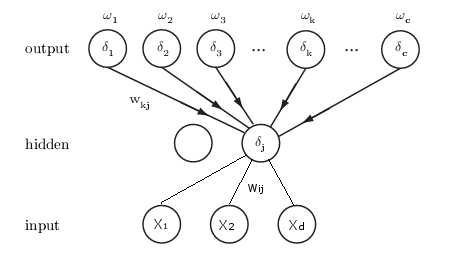
\includegraphics[width=7.5cm]{./images/backpropagation.png}
 \end{minipage}\\
 
 \begin{minipage}{8cm}
 \skriptsubsubsubsection{Variants}{293}
 \begin{liste}
   \item Input units include a bias unit. (very often)
   \item There are different non-linearities for different layers
   \item There are more than three layers. (the process works similar to the steps 3 \& 4)
   \item Input units are connected directly to output units as well as to hidden units
   \item Each unit has its own non-linearity
   \item Each unit has a different learning rate
 \end{liste}
 
 \end{minipage}
 \begin{minipage}{10cm}
 \skriptsubsubsubsection{Training Protocols}{293}\\
 There are different variant how to present the training set to the algorithm:\\
 \begin{liste}
   \item The \em Stochastic Training \em is the most common variant. The training sample are chosen randomly out of the training set\\
   \item In \em On-Line Training \em the training pattern are presented only once. So no memory for storing are used. An example of this variant is the frog algorithm from Guido\\
   \item The \em Batch training \em is not really common. Here all training data were presented before take one update.\\
 \end{liste}
 \end{minipage}
 
 \begin{minipage}{10cm}
 \skriptsubsubsubsection{Stopping Criterion}{295}\\
 To avoid overfitting, after every epoch (train all training sample one time) validation is done with a small set of data.
 This data set has to be separated from the training samples.
 If the validation is going to be worse, the training has to be stopped.\\
 
 After stopping a test has to decide if the result is good enough. For this a bigger data set (again separated from the training data) is tested and 
 the total error $\bm J = \sum\limits_{p=1}^n \bm J_p$ has to be low enough.
 \end{minipage}
 \hspace{5mm}
 \begin{minipage}{8cm}
 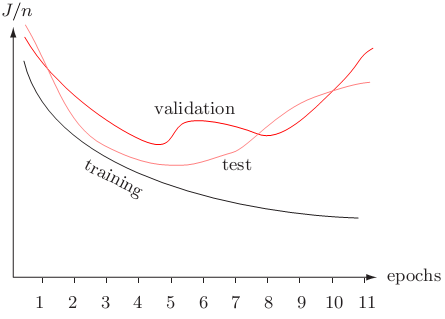
\includegraphics[width=7.5cm]{./images/stopCriterion.png}
 \end{minipage}
 

 \skriptsubsection{Activation Function}{307}
 $$ f(net)=a \tanh(b \cdot net)= a \left[\frac{e^{b\cdot net}-e^{-b \cdot net}}{e^{b\cdot net}+ e^{-b\cdot net}}\right]$$
  The sigmoid is a function which is non-linear, continuous, differentiable, monotonous, smooth and saturating. Its maximum steepness is at 0.
  
  \begin{center}
      \begin{tikzpicture}
\begin{groupplot}[
    group style={
        group size=3 by 1,
    },
    footnotesize,
    width=5cm,
    height=4cm,
    tickpos=left,
    ytick align=outside,
    xtick align=outside,
    enlarge x limits=false 
]

\nextgroupplot[title={$f(\mathrm{net})$}]
\addplot[blue,domain=-4:4,samples=201] {1.716*tanh(2/3*x)};
\nextgroupplot[title={$f'(\mathrm{net})$}]
\addplot[blue,domain=-4:4,samples=201] {(4*1.716*2/3*cosh(2/3*x)^2)/(cosh(4/3*x)+1)^2};
\nextgroupplot[title={$f''(\mathrm{net})$}]
\addplot[blue,domain=-4:4,samples=201] {-(8*1.716*4/9*sinh(4/3*x)*cosh(2/3*x)^2)/(cosh(4/3*x)+1)^3};

\end{groupplot}

\end{tikzpicture}
  \end{center}
    
  \skriptsubsubsection{Parameters}{308}
  It is important to choose the parameters for the sigmoid carefully. The factor $a$ defines the maximum output of an node.
  It should be bigger than the maximum of the needed output. A common value is $1.716$ if the output is normalized to $1$.
  If $a$ is to large, the sigmoid function is almost linear and if $a$ is to small, the function is in saturation and the target won't be reached or just to slowly.
  If $b=2/3$ is chosen, the maximum of the first derivation is 1 and and that the linear range is $\approx -1 < net < +1$ 
  \subsubsection{Scaling Input}
  The input (training and test samples) has often be scaled / standardize. The variance and the mean over \textbf{all} trainings sample should be: 
  $\sigma^2=1$ and $\mu=0$. The same factors as used for the training data has to be used for operation.
  
  
 \skriptsubsection{Techniques for Improving Backpropagation}{309}
 
 \skriptsubsubsection{Training with Noise}{310}
 To have more training samples, the true training samples can be added with d-dimensional Gaussian noise.
 If the training samples were standardized the variance has to be less than 1 (e.g. 0.1) and the category label should be left unchanged.
 
 \skriptsubsubsection{Number of Hidden Units}{310}
 When the number of hidden units is too low, the performance is probably too low, but a high number 
 increases the danger of overfitting. A rule of thumb is $n_H = n/10$ with $n$ as the number of training samples.
 
 \skriptsubsubsection{Learning Rates}{312}
 The training rates $\eta$ does not have to be constant. In general,  $\eta < 2\eta_{opt}$ with $\eta_{opt}= \left( \frac{\partial^2\bm J}{\partial w^2} \right)^{-1}$ (Newton). 
 A first choice can be $\eta \approx 0.1$ or $\eta \approx 0.01$.
 
 \skriptsubsubsection{Momentum}{313}
 The momentum is a kind of lowpass filtering of the update direction. So not only the current update value is used also the last one:\\
 $\bm w(m+1)= \bm w(m) +(1-\alpha) \Delta\bm w_{bp}(m) + \alpha \Delta \bm w(m-1)$ with $\alpha \approx 0.9$.
 
 \skriptsubsubsection{Weight Decay}{314}
 Before updating the weight vectors they are made a bit smaller $\bm w_{new}= \bm _{old}(1-\epsilon)$. 
 This has the effect that rare (unimportant) but big samples slowly eliminated and the often/important but small vectors are counted more.
 
 \skriptsubsubsection{Hint}{315}
 The idea is to give during the training additional knowledge into the algorithm with additional output nodes. For the test this nodes are ignored. 
 One example could be the frog, where the training is also given in which quadrant the fly is.
 

 \skriptsubsection{Backpropagation as Feature Mapping}{299}
  In a neural network with one hidden layer, the outputs $y_i$ of the hidden layer can be interpreted as nonlinearly mapped features.
  The output layer then classifies based on these mapped features. 

 \skriptsubsection{Backpropagation, Bayes Theory and Probability}{303}
 Shows that neural networks approximate the a \emph{posteriori probability}.
 
